\documentclass{ximera}

\author{Bart Snapp}

\title{Intersecting planes}

\begin{document}
\begin{abstract}
  One group member will plot intersecting planes.
\end{abstract}
\maketitle

One group member will produce a plot like this one:
\begin{image}
  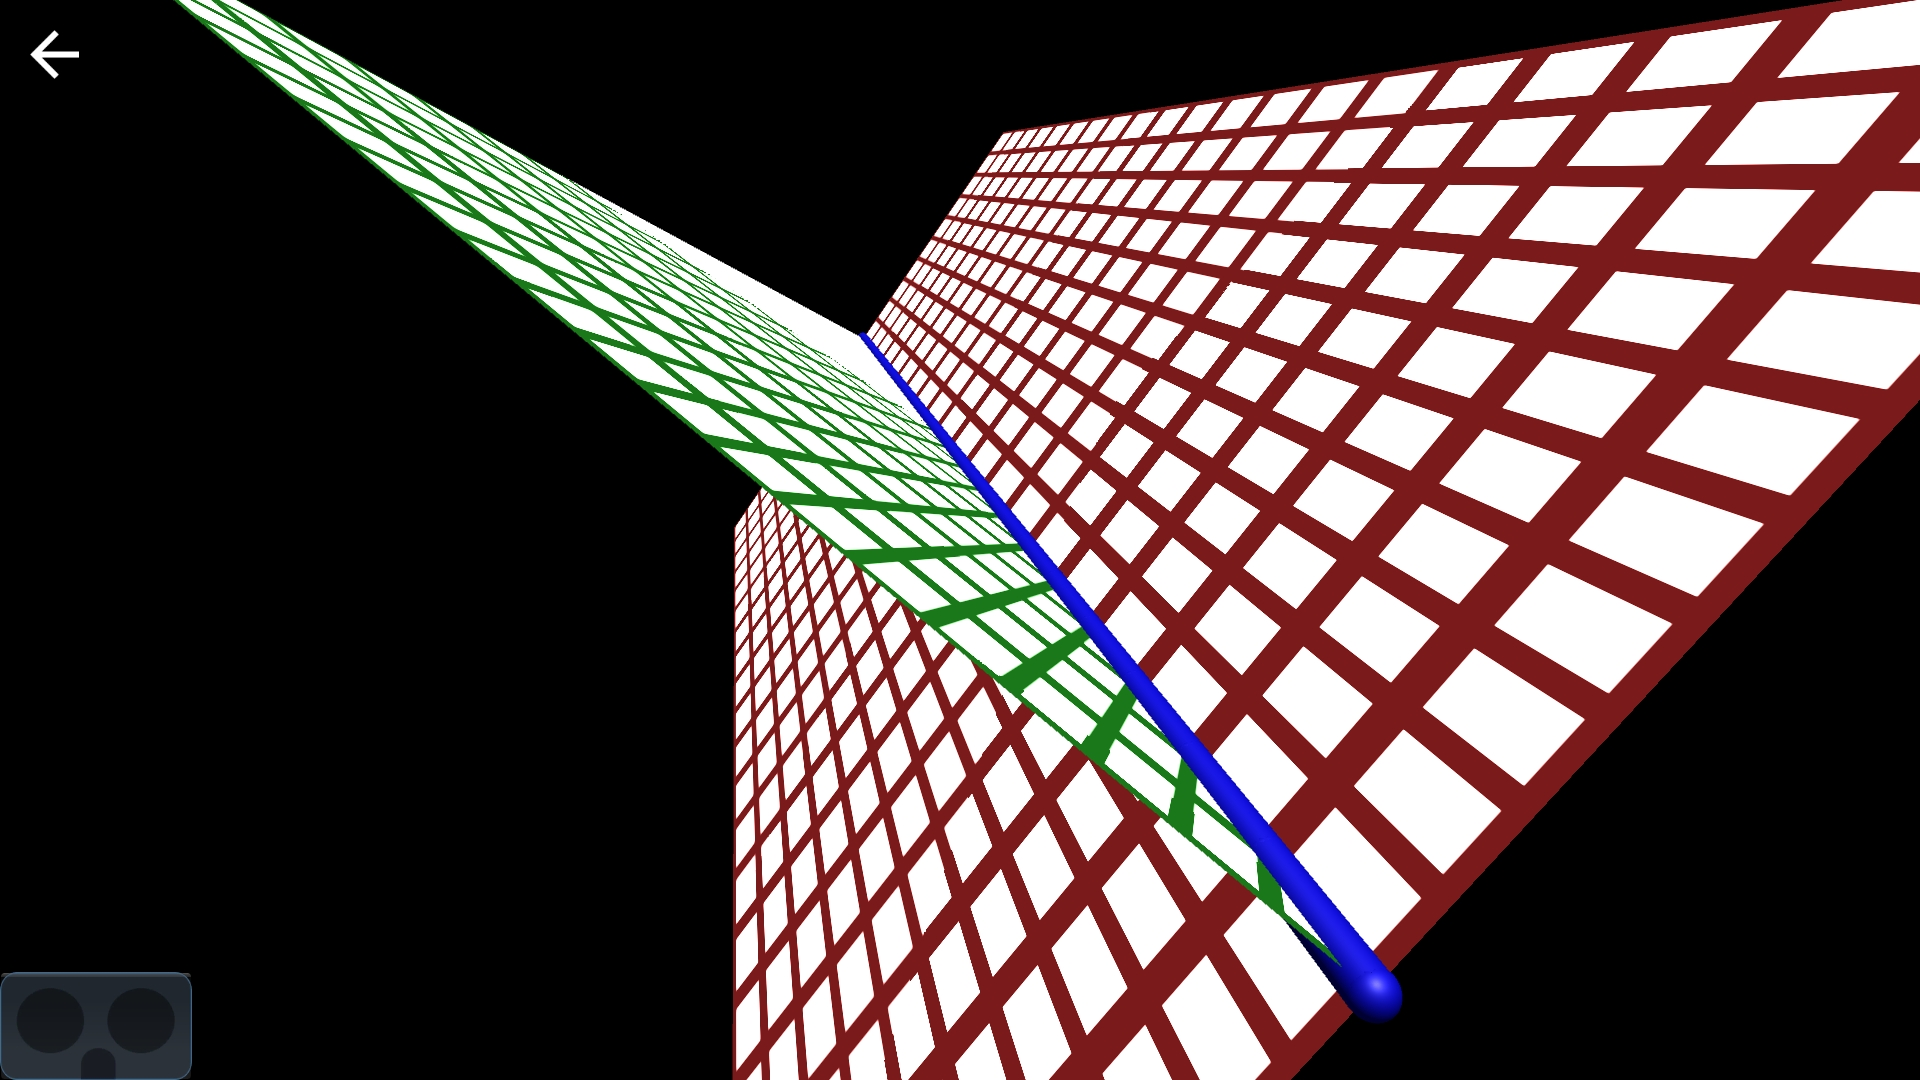
\includegraphics{intersection.png}
\end{image}

This is the intersection of the planes
\[
-x-y+z=1\quad\text{and}\quad  x+z=1
\]
along with a line at the intersection. You may make the line any
color you wish.
\end{document}
